\documentclass{article}

% if you need to pass options to natbib, use, e.g.:
% \PassOptionsToPackage{numbers, compress}{natbib}
% before loading nips_2018

% ready for submission
% \usepackage{nips_2018}

% to compile a preprint version, e.g., for submission to arXiv, add
% add the [preprint] option:
 \usepackage[preprint]{nips_2018}

% to compile a camera-ready version, add the [final] option, e.g.:
% \usepackage[final]{nips_2018}

% to avoid loading the natbib package, add option nonatbib:
% \usepackage[nonatbib]{nips_2018}

\usepackage[utf8]{inputenc} % allow utf-8 input
\usepackage[T1]{fontenc}    % use 8-bit T1 fonts
\usepackage{hyperref}       % hyperlinks
\usepackage{url}            % simple URL typesetting
\usepackage{booktabs}       % professional-quality tables
\usepackage{amsfonts}       % blackboard math symbols
\usepackage{nicefrac}       % compact symbols for 1/2, etc.
\usepackage{microtype}      % microtypography
\usepackage{graphicx}
\usepackage{verbatim}

\title{CS760 Project Proposal: Data driven prediction of droplet collision outcomes}

% The \author macro works with any number of authors. There are two
% commands used to separate the names and addresses of multiple
% authors: \And and \AND.
%
% Using \And between authors leaves it to LaTeX to determine where to
% break the lines. Using \AND forces a line break at that point. So,
% if LaTeX puts 3 of 4 authors names on the first line, and the last
% on the second line, try using \AND instead of \And before the third
% author name.

\author{
  Arpit Agarwal\thanks{I will be working alone towards this project. I have explained my reasons in section~\ref{sec:proposal}.} \\
  %Department of Mechanical Engineering\\
  %University of Wisconsin -- Madison\\
  \texttt{agarwal32@wisc.edu} \\
  %% examples of more authors
  %% \And
  %% Coauthor \\
  %% Affiliation \\
  %% Address \\
  %% \texttt{email} \\
  %% \AND
  %% Coauthor \\
  %% Affiliation \\
  %% Address \\
  %% \texttt{email} \\
  %% \And
  %% Coauthor \\
  %% Affiliation \\
  %% Address \\
  %% \texttt{email} \\
  %% \And
  %% Coauthor \\
  %% Affiliation \\
  %% Address \\
  %% \texttt{email} \\
}

\begin{document}
% \nipsfinalcopy is no longer used

\maketitle

\begin{abstract}
  Collision of liquid droplets is an important, and extensively studied phenomenon, but current physics based models for predicting the outcome are poor ($\approx 65\%$ accuracy). The models suffer because they are only able to account for 3 features, while there are many more important features that go unaccounted for. This limitation of traditional models is actually a strength of ML based models which will benefit from a higher number of input features. This makes the problem of classifying outcomes of droplet collisions very suitable for ML based modeling. Here I propose to implement ML based classifiers that will greatly improve the accuracy from the current state of the art fluid mechanistic models.
\end{abstract}

\section{Motivation}
Droplet collisions are important to the dynamics of a liquid spray. Sprays of engineering relevance have a very high droplet density and therefore a lot of droplet collisions. For example, diesel sprays have been reported to have 10$^8$  collisions per cm$^3$ per microsecond. Collisions have a direct effect on the liquid drops as they change the droplet sizes and velocities. Due to the high frequency of droplet collisions, and their cascading effect on the system dynamics, it is important to accurately model the droplet collision phenomena.

The problem of modeling the outcome of droplet collisions has been worked on extensively by fluid dynamicists. The models proposed in literature for predicting the outcomes of droplet collisions are phenomenological. They are based simplified analyses of the governing fluid dynamics equations. The present models correctly predict the outcome for around 65\% of the instances. The complexity of these models is limited by our understanding of fluid mechanics, and our cognitive limitations. More complex models are needed to improve the accuracy.

In this work I will collate some labelled datasets from literature (2,000 to 2,500 data points are available in all). Using this data I will generate machine learning based classification models for predicting the outcome of the collisions.

\section{Background}
Four main types of outcomes are expected from collisions of two droplets, these are illustrated in figure~\ref{fig:outcomes}. A priori prediction of collision outcomes is possible with enough information about the droplet and flow characteristics. Due to limitations of the techniques used, in current fluid mechanics literature, only three main non-dimensional quantities, $\Delta, We_D$ and $B$ are considered in the outcome of a binary collision. It is well known that more features are relevant, but no models exist that account for all relevant features.

\begin{figure}
	\centering
	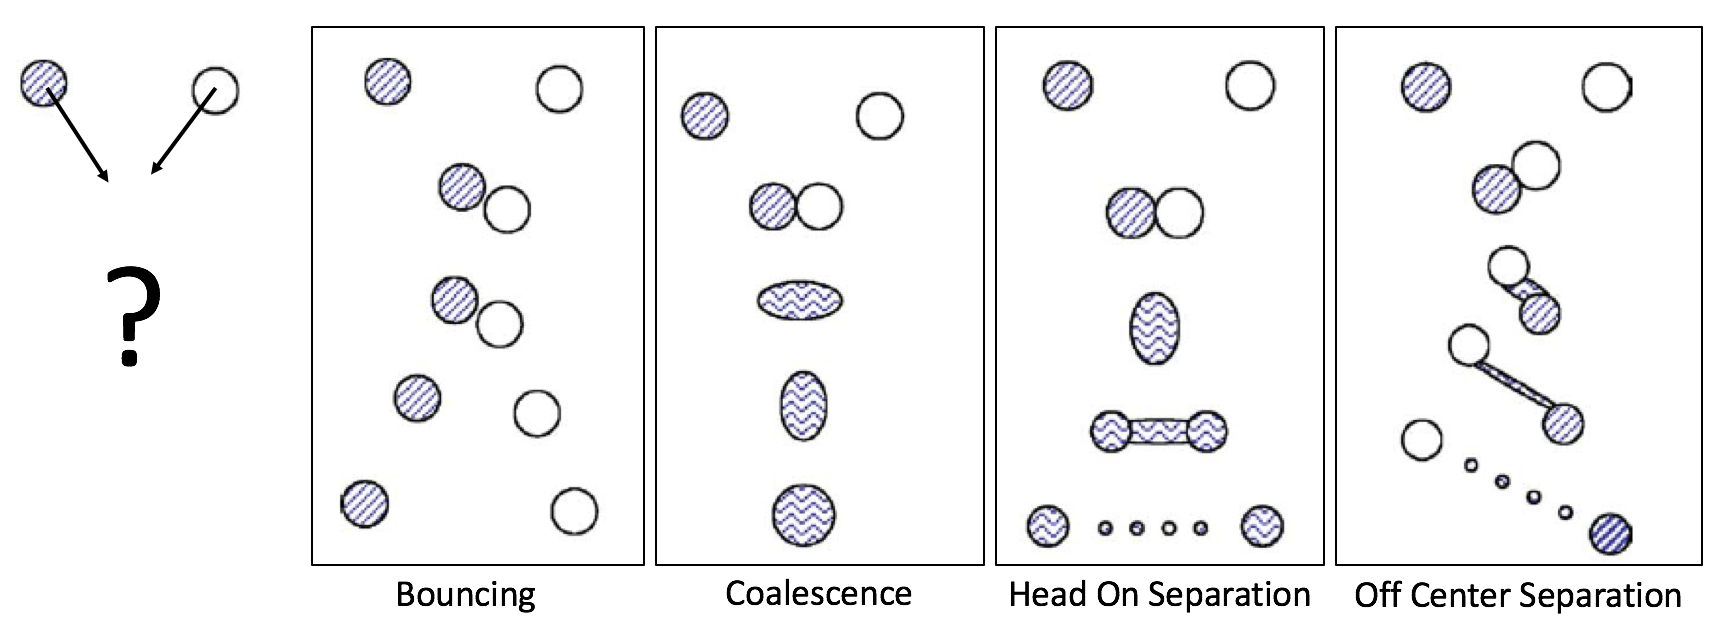
\includegraphics[width=0.8\textwidth]{../figures/outcome-illustration.png}
	\caption{An illustration of the 4 types of outcomes expected. These are the classification labels for the present study.}
	\label{fig:outcomes}
\end{figure}

As per the traditional modeling approach, the 3-dimensional feature space is divided into 4 regions corresponding to the respective outcomes. Figure~\ref{fig:munnannur} shows a slice of this 3-dimensional space ($\Delta$ is set to 1), showing the four different outcomes. This figure also gives an example of a typical labelled experimental dataset. For this project I will compile many such sets, amounting to 2,000 to 2,500 data points.

\begin{figure}[h]
	\centering
	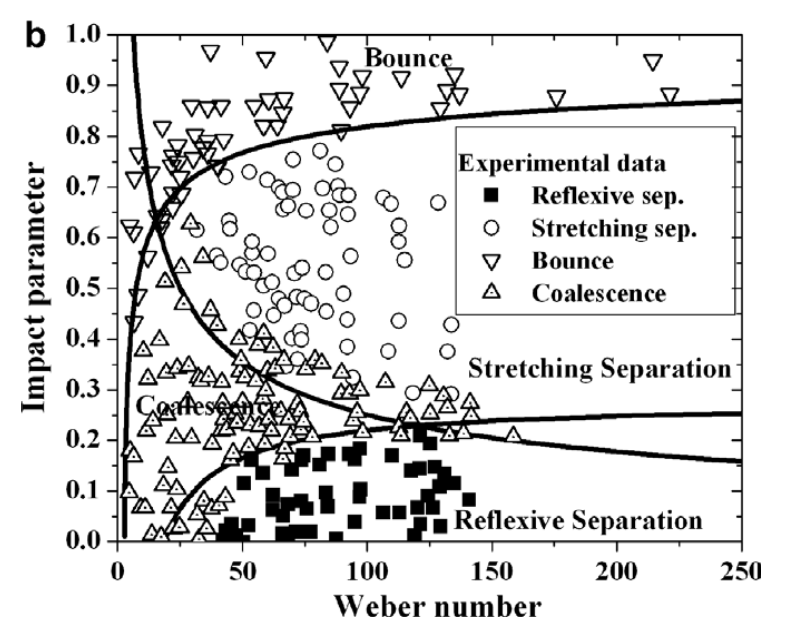
\includegraphics[width=0.5\textwidth]{../figures/munnannur.png}
	\caption{A sample dataset with the 4 labels and the traditional (fluid-mechanistic) classification curves. These simplified curves fail to capture all of the physics (they only consider 3 features) and hence perform poorly.}
	\label{fig:munnannur}
\end{figure}

\section{Proposal}
\label{sec:proposal}
I propose to go about this project in steps as listed here:
\begin{itemize}
\item \textbf{Data collection (present to Nov. 16)}: The data has been reported by different researchers over the last 4-5 decades. I will collect this data and put it in a workable format.
\item \textbf{Missing data handling (present to Nov. 16)}: Not all datasets report all the features, I will figure out techniques of filling the gaps or some other way of handling the missing data.
\item \textbf{Expanding from 3 features (Nov. 16 - Nov. 23)}: This is the main reason for leveraging ML models for this problem. There are at least 9 independent features and numerous other combinations of these base features that actually affect the collision phenomenon. Traditional fluid mechanics models are limited to 3 features, while the ML models have no such limitation. Using my domain specific knowledge, I will generate a list of all possible features that might be relevant here.
\item \textbf{Implementation (Nov. 16 - Nov. 23)}: Using libararies like scikit-learn, tensorflow etc. I will implement linear and non-linear classifiers like decision trees, k-nearest neighbors, neural networks, bayesian-networks etc.
\item \textbf{Analysis (Nov. 30 - Dec. 7)}: Through cross validation, I will optimize the hyper-parameters. I will compare the different models with respect to the present dataset.
\item \textbf{Instructing traditional models (Dec 7 onwards)}: Based on the ML models, I will then try to see if we can learn anything about the physics of the collision phenomenon and hence instruct traditional models.
\end{itemize}

I am working alone on this project mainly because this topic is very narrow and related to my area of research. I work on fluid mechanics research in the Department of Mechanical Engineering. This problem is exciting to me as there is a very clear need and a possibility of great improvement here. This could directly help improve fluid mechanics simulations in industry. I could not find anyone else who wanted to work on this problem.


\begin{comment}
\begin{enumerate}
\item Drop size ratio, $\Delta = d_s/d_l$,  where $d_s$ and $d_l$ are the diameters of the smaller and larger participating drops, respectively
\item	Drop Weber number, $We_D = \rho U^2 d_s/\sigma$, where $\rho, U$ and $\sigma$ are the liquid density, relative velocity and surface tension constant respectively
\item Impact parameter, $B$, which is the non-dimensionalized orthogonal distance between the interacting drops. It has been described in further detail in [8].
\end{enumerate}
\end{comment}

\clearpage
\begin{figure}[h]
	\centering
	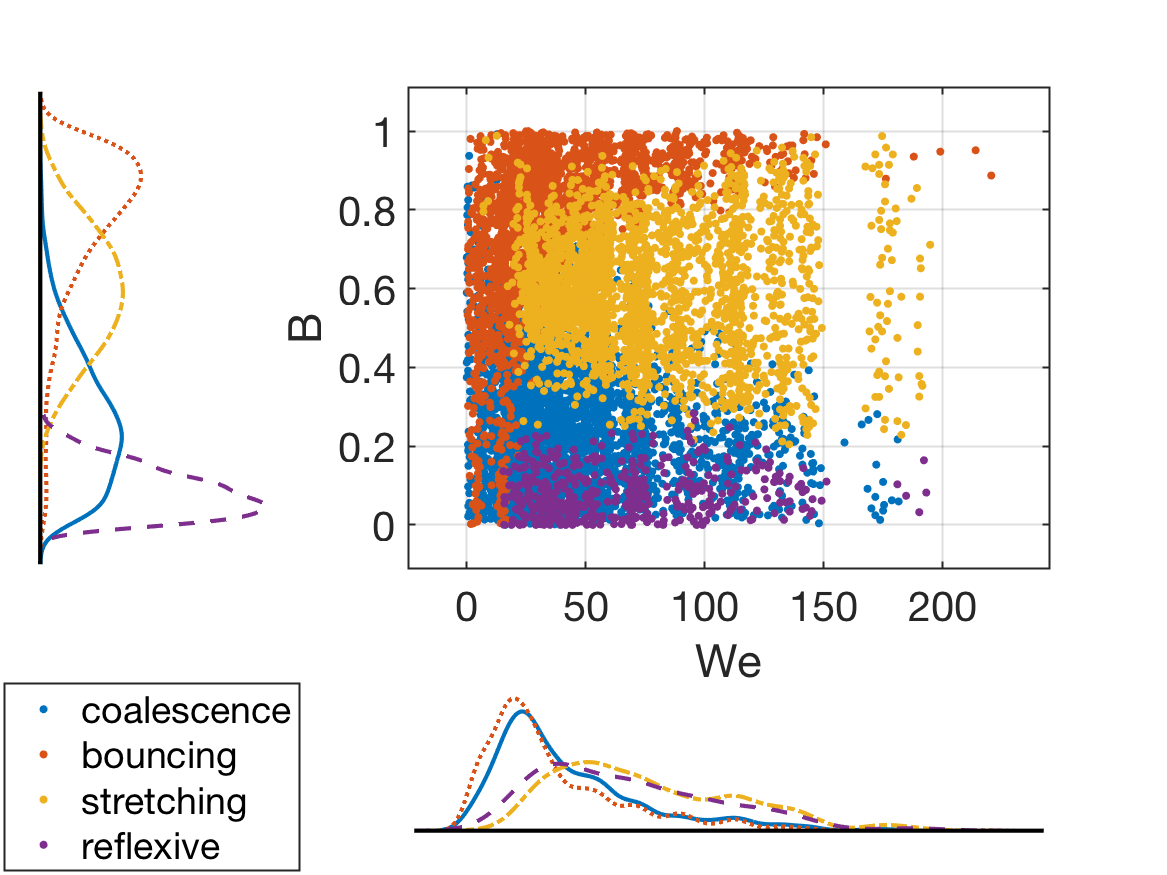
\includegraphics[width=0.95\textwidth]{../figures/data_scatterhist.png}
	\caption{Data}
	\label{fig:data}
\end{figure}

\section{ML Models}
\subsection{Decision Trees}
\begin{figure}[h!]
	\centering
	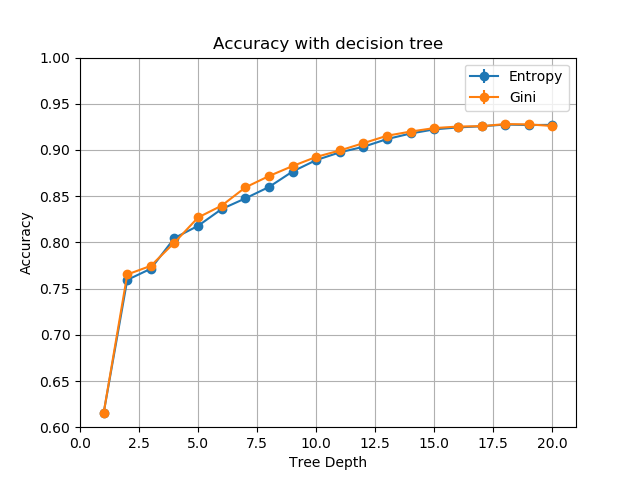
\includegraphics[width=0.6\textwidth]{../figures/accuracy_decision_tree.png}
	\caption{Accuracy with decision trees}
	\label{fig:dt}
\end{figure}

\subsection{K-Nearest Neighbors}
\begin{figure}[h!]
	\centering
	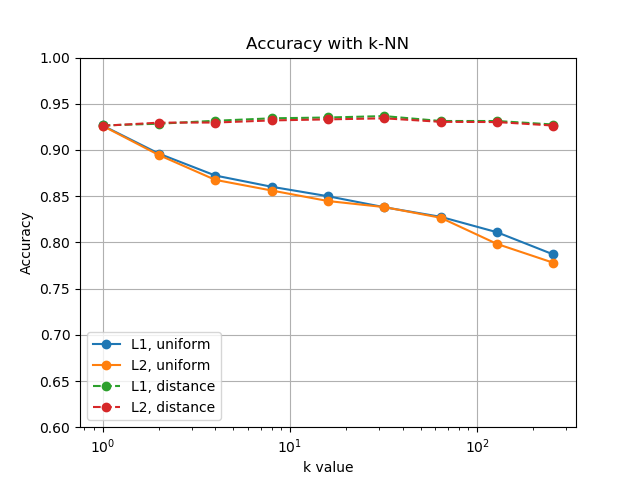
\includegraphics[width=0.6\textwidth]{../figures/accuracy_knn.png}
	\caption{Accuracy with k-nn}
	\label{fig:dt}
\end{figure}

\end{document}
